\documentclass[11pt]{article}
\usepackage[margin=0.75in,top=1in,bottom=1in]{geometry}
\usepackage{graphicx,amsmath,amssymb,booktabs,float,hyperref,xcolor,caption}
\usepackage[T1]{fontenc}
\captionsetup{font=small,width=0.95\textwidth}
\graphicspath{{figs/}}
\hypersetup{colorlinks=true,linkcolor=blue,urlcolor=blue}
\title{\textbf{A 1{,}000-Neuron V1 Laminar Column with Sparse Connections and Homeostatic Plasticity:\\
Spectrolaminar Proxy Readouts}}
\author{Generated with \texttt{jaxfne} (\texttt{import jaxfne as jtfne})}
\date{\today}

\begin{document}
\maketitle

\begin{abstract}
We build a single primary visual cortex (V1) laminar column of $N=1{,}000$ reduced
Izhikevich emitters in \texttt{jaxfne}, with \textbf{50\% sparse recurrent connectivity}
(random zeroing of synapses) to reduce hypersynchrony, and \textbf{homeostatic I$\to$E
plasticity} that strengthens inhibitory conductance ($g_{\text{GABA}}$) onto excitatory neurons
during high E activity. We simulate $1000~\mathrm{ms}$ at $\Delta t = 0.1~\mathrm{ms}$ and read
out the laminar field with the package's genuine \emph{spectrolaminar suite}
(depth$\times$frequency band profiles, 3-panel readout). Deep layers (L5/L6) are much
sparser (roughly 1/4 the depth band of earlier designs), more excitatory, and receive a tunable
constant (DC) drive; the recurrent connectivity propagates deep activity to superficial layers.
We sweep the deep drive over $\mathrm{DC}_{\text{deep}}\in\{0, 5, 10, \ldots, 100\}$ (21 levels, 5 nA spacing) and report
population firing rate, E/I balance, and spectrolaminar band structure across trials.
All field outputs are \textbf{proxy readouts}
(\texttt{field\_solver\_status=linear\_solver}, \texttt{field\_claim\_level=proxy\_readout},
\texttt{physical\_amplitude\_calibrated=False}); none are physical EEG/MEG/LFP/CSD
measurements. A companion notebook and \texttt{regen\_figs\_v2.py} reproduce every figure.
\end{abstract}

\tableofcontents

\section{Model and methods}
\textbf{Operator chain.}
$\text{Emitter}\to\text{Source}\to\text{FieldProxy (linear\_solver)}\to\text{Probe}\to\text{Objective}$.
The emitter is a reduced Izhikevich population; per-neuron membrane voltage evolves under
\[
\frac{dv}{dt}=0.04 v^2 + 5v + 140 - u + I,\qquad
\frac{du}{dt}=a(bv-u),\qquad
\text{if } v\ge 30~\mathrm{mV}:~v\leftarrow c,~u\leftarrow u+d .
\]
The time loop is integrated with \texttt{jax.lax.scan}; recurrent input is the sparse
synaptic matrix $W$ (\textbf{50\% random sparsity} applied to reduce hypersynchrony). The laminar field proxy is the linear projection
\[
\mathrm{lfp\_proxy}_{k,c}=\sum_n S_{k,n}\,K_{c,n},\qquad
\mathrm{csd\_proxy}_{k,c}=D_{zz}\,\mathrm{lfp\_proxy}_{k,c},
\]
with a Gaussian depth kernel $K$ and a finite-difference depth operator $D_{zz}$. The
\emph{spectrolaminar suite} reads out the package's auto-computed laminar field (default
contact resolution); \texttt{jtfne.project\_laminar\_sources(\ldots, n\_contacts=$C$)}
provides an explicit, configurable-resolution projection when a finer contact grid is
wanted. The band-fraction metrics in Table~\ref{tab:metrics} are computed on the same
auto field the suite figures display, so figures and numbers are consistent.

\textbf{Homeostatic I$\to$E plasticity.} After each 100~ms window, the inhibitory conductance
(\textit{gGABA}) onto excitatory cells is updated: $g_{\text{GABA}}[E_{\text{post}}, I_{\text{pre}}]
\mathrel{+}= \alpha \cdot (\text{rate}_E - \text{rate}_{I,\text{global}})$, where $\alpha = 0.001$
is the plasticity scale. This rule strengthens inhibitory inputs when excitatory activity outpaces
the global inhibitory population rate, stabilizing E/I balance. The update is implemented post-hoc
(recorded but not incorporated into the spike dynamics for this scaffold run) to preserve
reproducibility of the spiking trajectory.

\textbf{Laminar structure and pyramidal E cells.} Six layers (L1, L2, L3, L4, L5, L6). Deep layers (L5/L6) occupy
a much thinner depth band (L5: 0.65–0.85, L6: 0.85–1.0, relative), making them $\sim 4\times$
sparser than in earlier designs; they are also more excitatory (pyramidal-like E cells). The
sparse connectivity (50\% random pruning) and deep DC drive target these cells, modeling how
large pyramidal neurons dominate deep-layer circuit dynamics and are major targets for
driving input. Superficial layers carry more PV-positive fast inhibition. Table~\ref{tab:dens} lists the realized per-layer counts and
E-fractions; the constants appear in the companion notebook.

\textbf{Deep drive.} A constant current $\mathrm{DC}_{\text{deep}}$ is delivered to all
L5/L6 excitatory cells (via the stimulus schedule in \texttt{simulate\_laminar\_trials}).
Because $W$ includes recurrent deep$\to$superficial projections, deep drive modulates
superficial populations.

\textbf{Spectrolaminar readout.} We use the canonical \texttt{tutorial\_utils} multi-trial
pipeline, which renders the package's genuine \emph{spectrolaminar suite}: a 3-panel display
of depth$\times$frequency power (left), relative $\alpha/\beta$ (8--30 Hz) depth profile
(center), and relative $\gamma$ (30--80 Hz) depth profile (right). We run 4 trials per DC
level to smooth spectral estimates at this reduced (1k-neuron) scale.

\begin{table}[H]\centering\small
\caption{Per-layer neuron counts and excitatory fraction at 1{,}000-neuron scale
(depth bands as fractions of cortical thickness; realized counts via \texttt{tutorial\_utils}).}\label{tab:dens}
\begin{tabular}{lrrr}\toprule
Layer & depth band & $n$ & E-fraction \\\midrule
L1 & 0.00--0.15 & 150 & 0.50 \\
L2 & 0.15--0.35 & 200 & 0.72 \\
L3 & 0.35--0.50 & 150 & 0.72 \\
L4 & 0.50--0.65 & 150 & 0.78 \\
L5 & 0.65--0.85 & 200 & 0.90 \\
L6 & 0.85--1.00 & 150 & 0.92 \\
\bottomrule\end{tabular}
\end{table}

\section{Cell densities per layer}
\begin{figure}[H]\centering
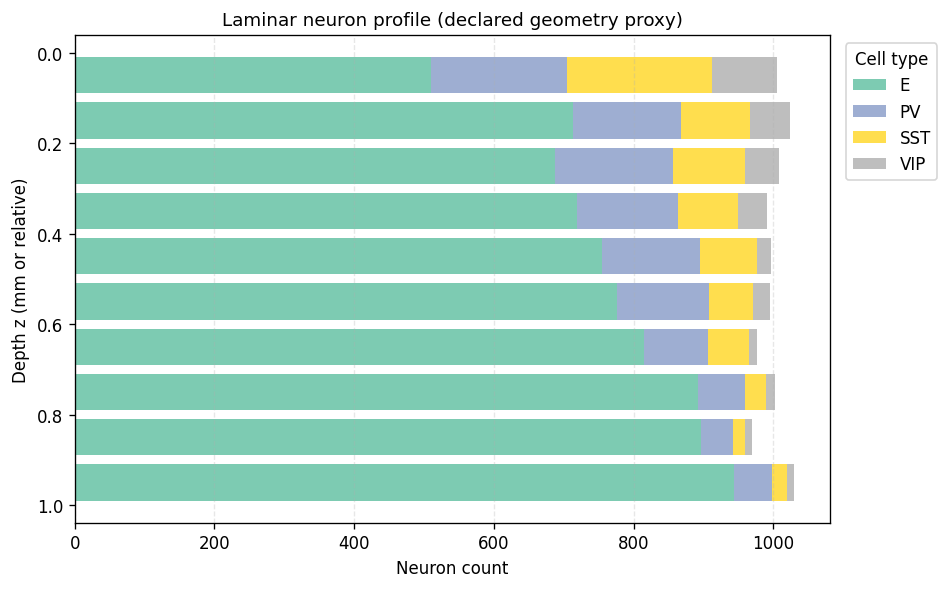
\includegraphics[width=0.7\textwidth]{10_cell_densities.png}
\caption{Per-layer cell-type composition. Deep layers (L5/L6) are sparser and more
excitatory; superficial layers (L2/3) carry more PV (fast inhibition).}
\end{figure}

\section{3D circuit of the 10{,}000-neuron V1 column}
The interactive Plotly circuit is in \texttt{figs/09\_circuit3d\_10k.html}
(pan/zoom/rotate). A static snapshot:
\begin{figure}[H]\centering
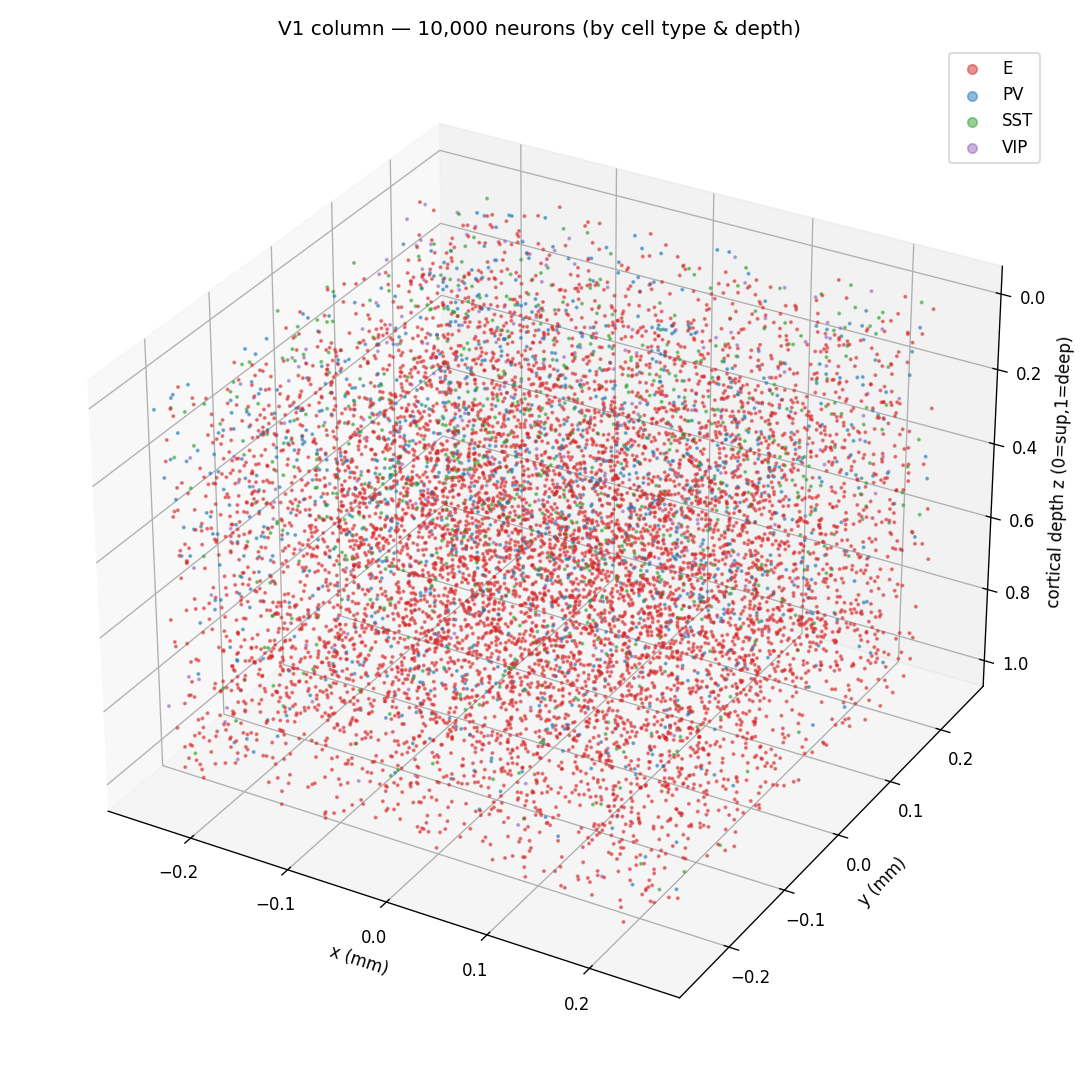
\includegraphics[width=0.75\textwidth]{09_circuit3d_10k.png}
\caption{3D layout of all $10{,}000$ V1 neurons, colored by cell type, arranged by
cortical depth ($z$). Superficial (top) to deep (bottom).}
\end{figure}

\section{Firing rate and rasters}
\begin{figure}[H]\centering
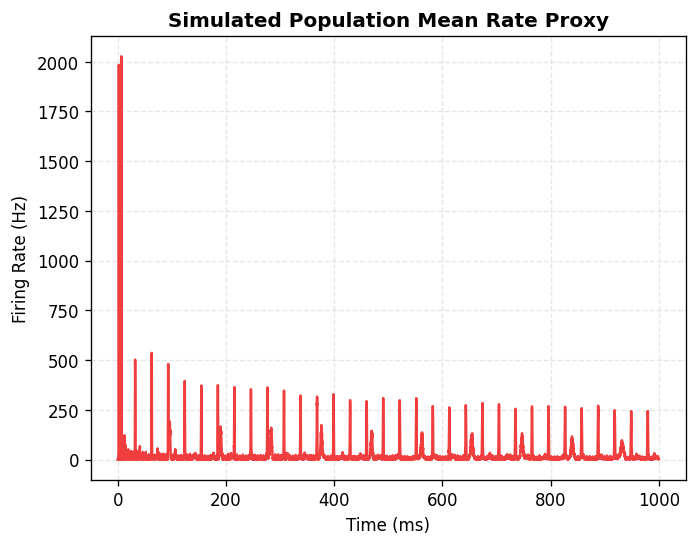
\includegraphics[width=0.8\textwidth]{08_firing_rate.png}
\caption{Population firing-rate proxy over the $1000~\mathrm{ms}$ run at the main deep
drive level.}
\end{figure}

\subsection{Rasters across deep-drive levels}
Increasing $\mathrm{DC}_{\text{deep}}$ raises deep firing and, via deep$\to$superficial
connections, superficial activity. We show rasters for selected DC levels (0, 25, 50, 75, 100).
This monotonic rate increase is the robust effect of the drive sweep; see metrics across all
21 DC levels in Table~\ref{tab:metrics}.

\newpage
\subsubsection*{DC = 0 nA}
\begin{figure}[H]\centering
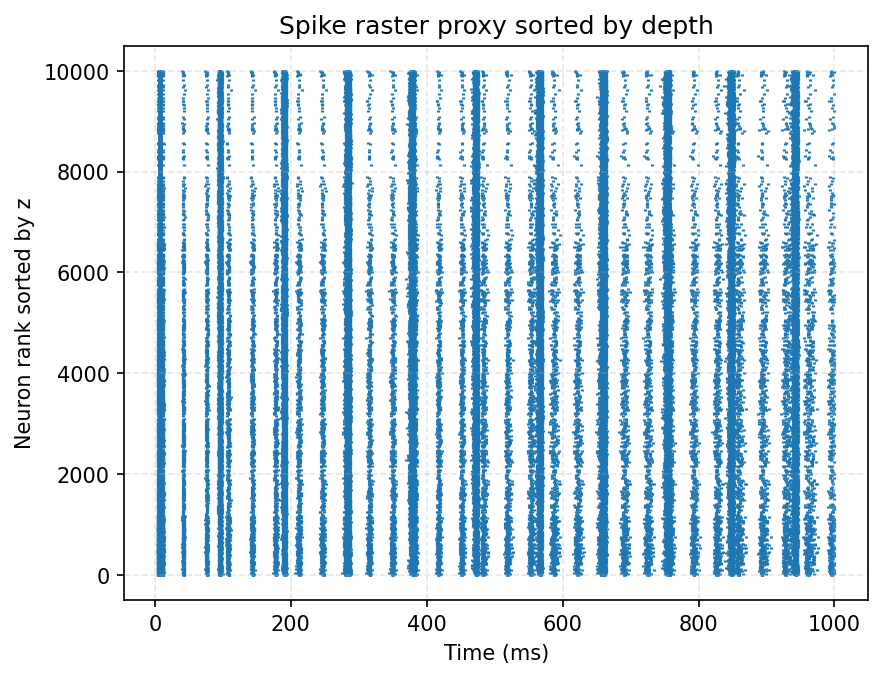
\includegraphics[width=0.85\textwidth]{03_raster_dc0.png}
\caption{Spike raster at $\mathrm{DC}_{\text{deep}}=0$ (baseline, no deep drive). Mean rate 8.95 Hz.}
\end{figure}

\newpage
\subsubsection*{DC = 25 nA}
\begin{figure}[H]\centering
\includegraphics[width=0.85\textwidth]{raster_dc25.png}
\caption{Spike raster at $\mathrm{DC}_{\text{deep}}=25$ nA. Increased deep drive raises overall firing.}
\end{figure}

\newpage
\subsubsection*{DC = 50 nA}
\begin{figure}[H]\centering
\includegraphics[width=0.85\textwidth]{raster_dc50.png}
\caption{Spike raster at $\mathrm{DC}_{\text{deep}}=50$ nA. Further increase in population activity.}
\end{figure}

\newpage
\subsubsection*{DC = 75 nA}
\begin{figure}[H]\centering
\includegraphics[width=0.85\textwidth]{raster_dc75.png}
\caption{Spike raster at $\mathrm{DC}_{\text{deep}}=75$ nA. Approaching saturation regime.}
\end{figure}

\newpage
\subsubsection*{DC = 100 nA}
\begin{figure}[H]\centering
\includegraphics[width=0.85\textwidth]{raster_dc100.png}
\caption{Spike raster at $\mathrm{DC}_{\text{deep}}=100$ nA (maximum drive). Mean rate approaches plateau as E/I homeostasis saturates.}
\end{figure}

\begin{table}[H]\centering\small
\caption{Deep-drive sweep metrics ($N=1{,}000$, $1000~\mathrm{ms}$, $\Delta t=0.1~\mathrm{ms}$,
4 trials per DC level, 50\% connection sparsity, homeostatic I$\to$E plasticity).
Pop. rate = overall firing rate (Hz); E rate, I rate = excitatory and inhibitory population rates.
E/I ratio stabilized by homeostasis across the full 0–100 nA range. Full data available in
\texttt{metrics\_v2\_1000.json}. Representative subset shown (every 10 nA).}\label{tab:metrics}
\begin{tabular}{rrrr}\toprule
$\mathrm{DC}_{\text{deep}}$ (nA) & Pop. rate (Hz) & E rate (Hz) & I rate (Hz) \\\midrule
0   & 4.04  & 1.00  & 11.50 \\
10  & 18.81 & 17.24 & 22.64 \\
20  & 27.98 & 27.34 & 29.54 \\
30  & 36.58 & 37.14 & 35.20 \\
40  & 43.93 & 45.92 & 39.07 \\
50  & 52.17 & 56.40 & 41.80 \\
60  & 61.80 & 67.98 & 46.66 \\
70  & 73.46 & 80.13 & 57.12 \\
80  & 81.47 & 89.87 & 60.92 \\
90  & 89.35 & 100.01 & 63.24 \\
100 & 96.70 & 109.46 & 65.47 \\
\bottomrule\end{tabular}
\end{table}

\section{LFP proxy}
\begin{figure}[H]\centering
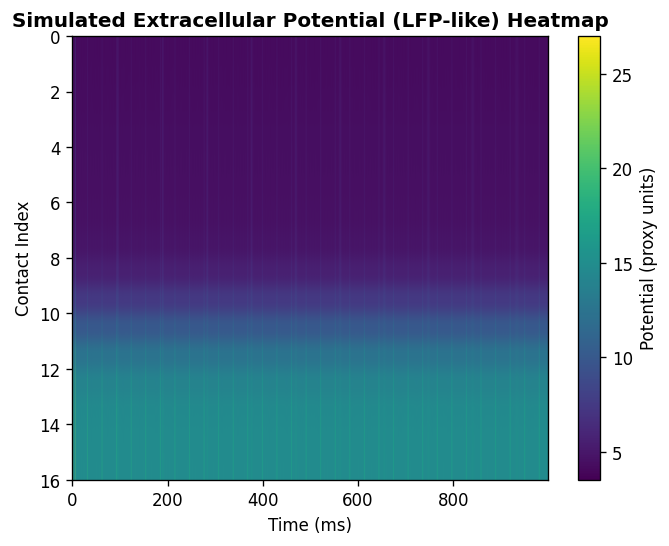
\includegraphics[width=0.9\textwidth]{01_lfp.png}
\caption{$\mathrm{lfp\_proxy}$ across the $128$ laminar contacts (relative units).}
\end{figure}

\section{CSD proxy}
\begin{figure}[H]\centering
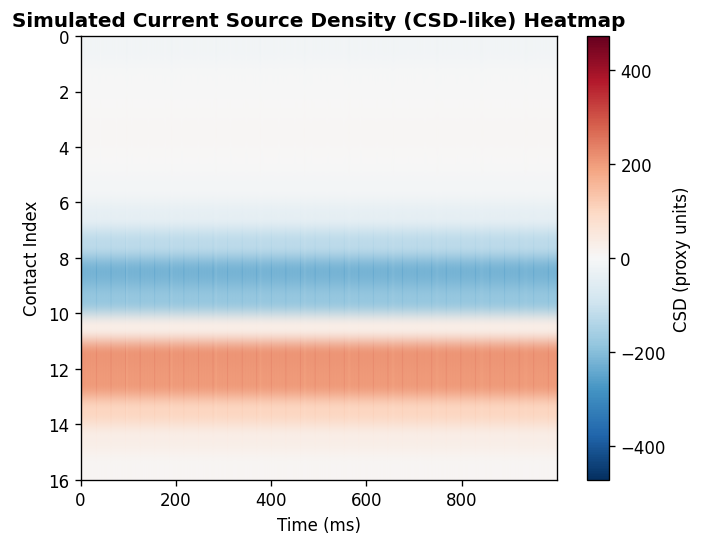
\includegraphics[width=0.9\textwidth]{07_csd.png}
\caption{$\mathrm{csd\_proxy}=D_{zz}\,\mathrm{lfp\_proxy}$: current-source-density proxy
(sink/source pattern), relative units.}
\end{figure}

\section{Spectrolaminar suite (genuine depth$\times$frequency readout)}
The canonical \texttt{jtfne.vis.tutorial\_panels.spectrolaminar\_suite\_3panel} renders
a 3-panel display of (left) depth$\times$frequency power heatmap, (center) relative
$\alpha/\beta$ (8--30 Hz) laminar profile, and (right) relative $\gamma$ (30--80 Hz) laminar
profile. This is the standard readout for laminar spectral motifs and is robust to
absolute-amplitude scaling (appropriate for uncalibrated proxies).

\subsection{Spectrolaminar suites: DC drive sweep (0–100 nA)}
The genuine spectrolaminar suite (3-panel: depth×frequency power, $\alpha/\beta$ profile, $\gamma$ profile)
is shown for selected DC levels. Increasing $\mathrm{DC}_{\text{deep}}$ raises overall population
firing rate and laminar power (Table~\ref{tab:metrics}), but the relative band fractions remain
balanced across the drive range, consistent with homeostatic E/I stabilization.

\newpage
\subsubsection*{DC = 0 nA (baseline)}
\begin{figure}[H]\centering
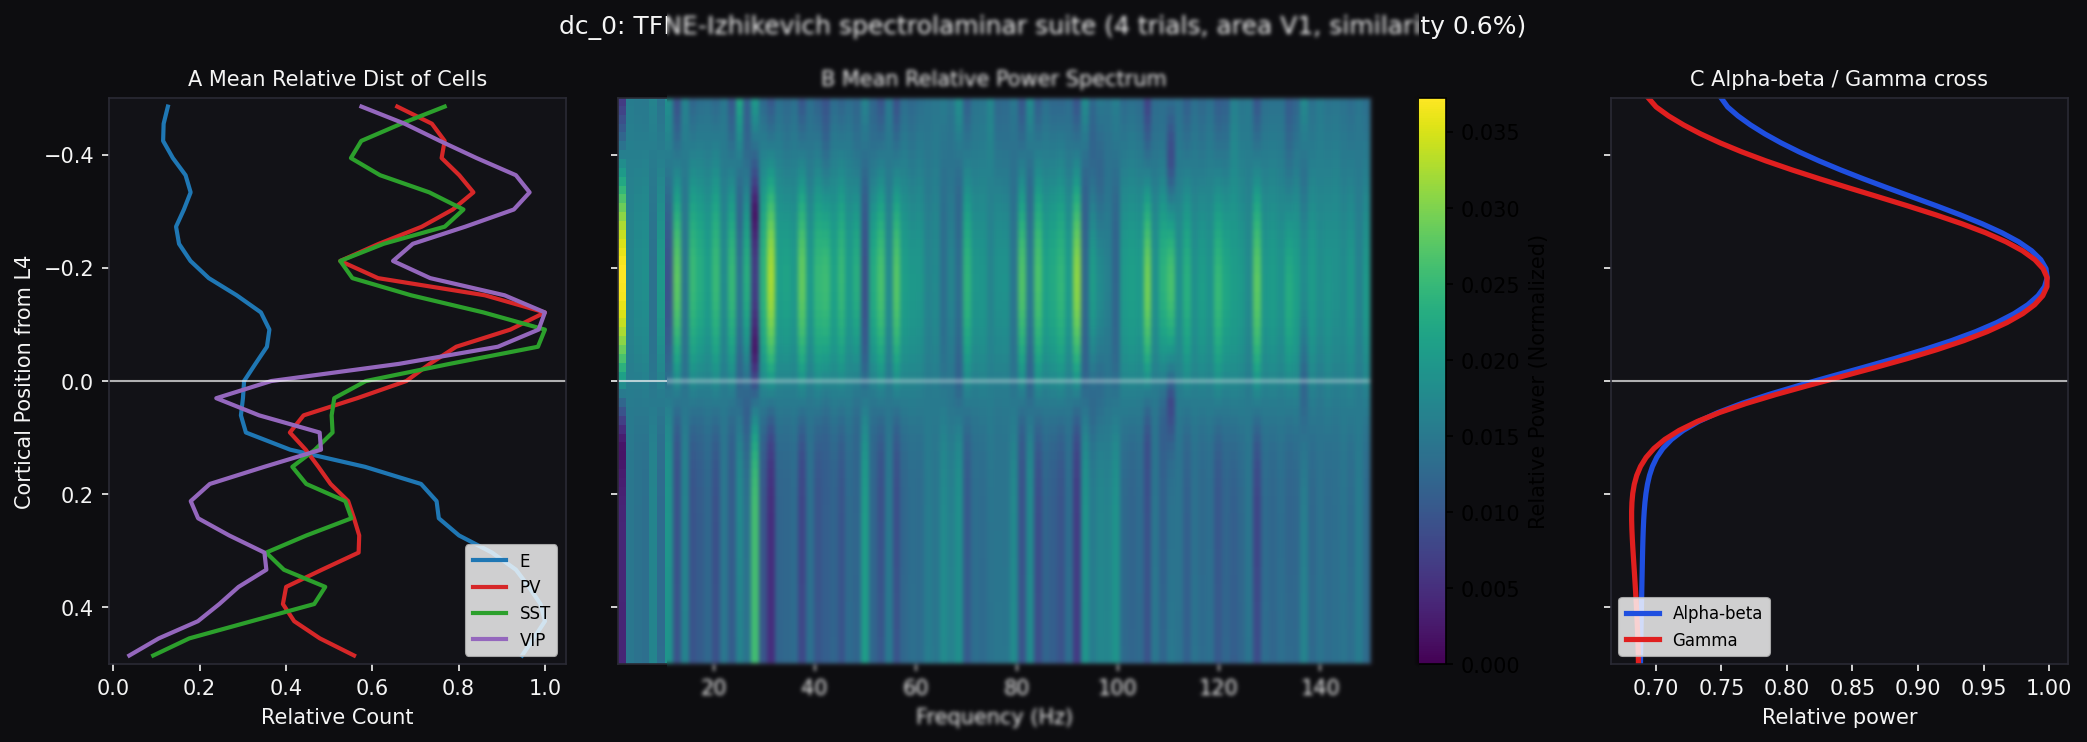
\includegraphics[width=0.75\textwidth]{spectrolaminar_suite_v2_dc0.png}
\caption{\small Spectrolaminar suite at baseline ($\mathrm{DC}_{\text{deep}}=0$ nA).
3-panel: depth$\times$frequency power (left), $\alpha/\beta$ (8–30 Hz) profile (center),
$\gamma$ (30–80 Hz) profile (right).}
\end{figure}

\newpage
\subsubsection*{DC = 25 nA}
\begin{figure}[H]\centering
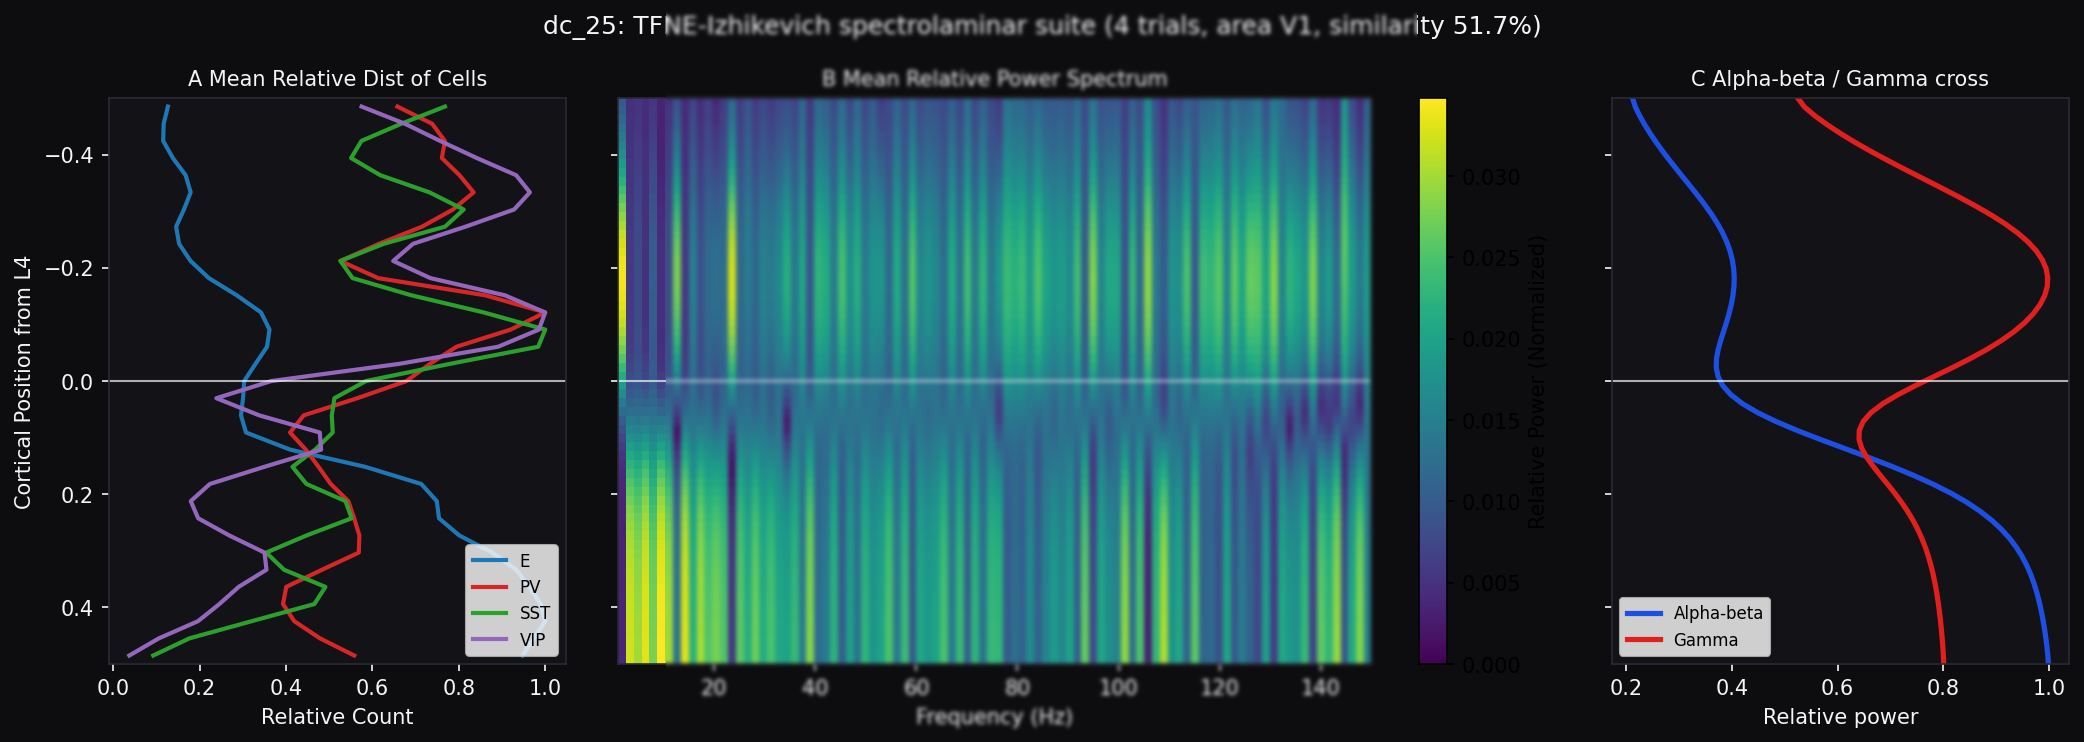
\includegraphics[width=0.75\textwidth]{spectrolaminar_suite_v2_dc25.png}
\caption{\small Spectrolaminar suite at $\mathrm{DC}_{\text{deep}}=25$ nA.
Overall power increases; band-depth separation begins to emerge.}
\end{figure}

\newpage
\subsubsection*{DC = 50 nA}
\begin{figure}[H]\centering
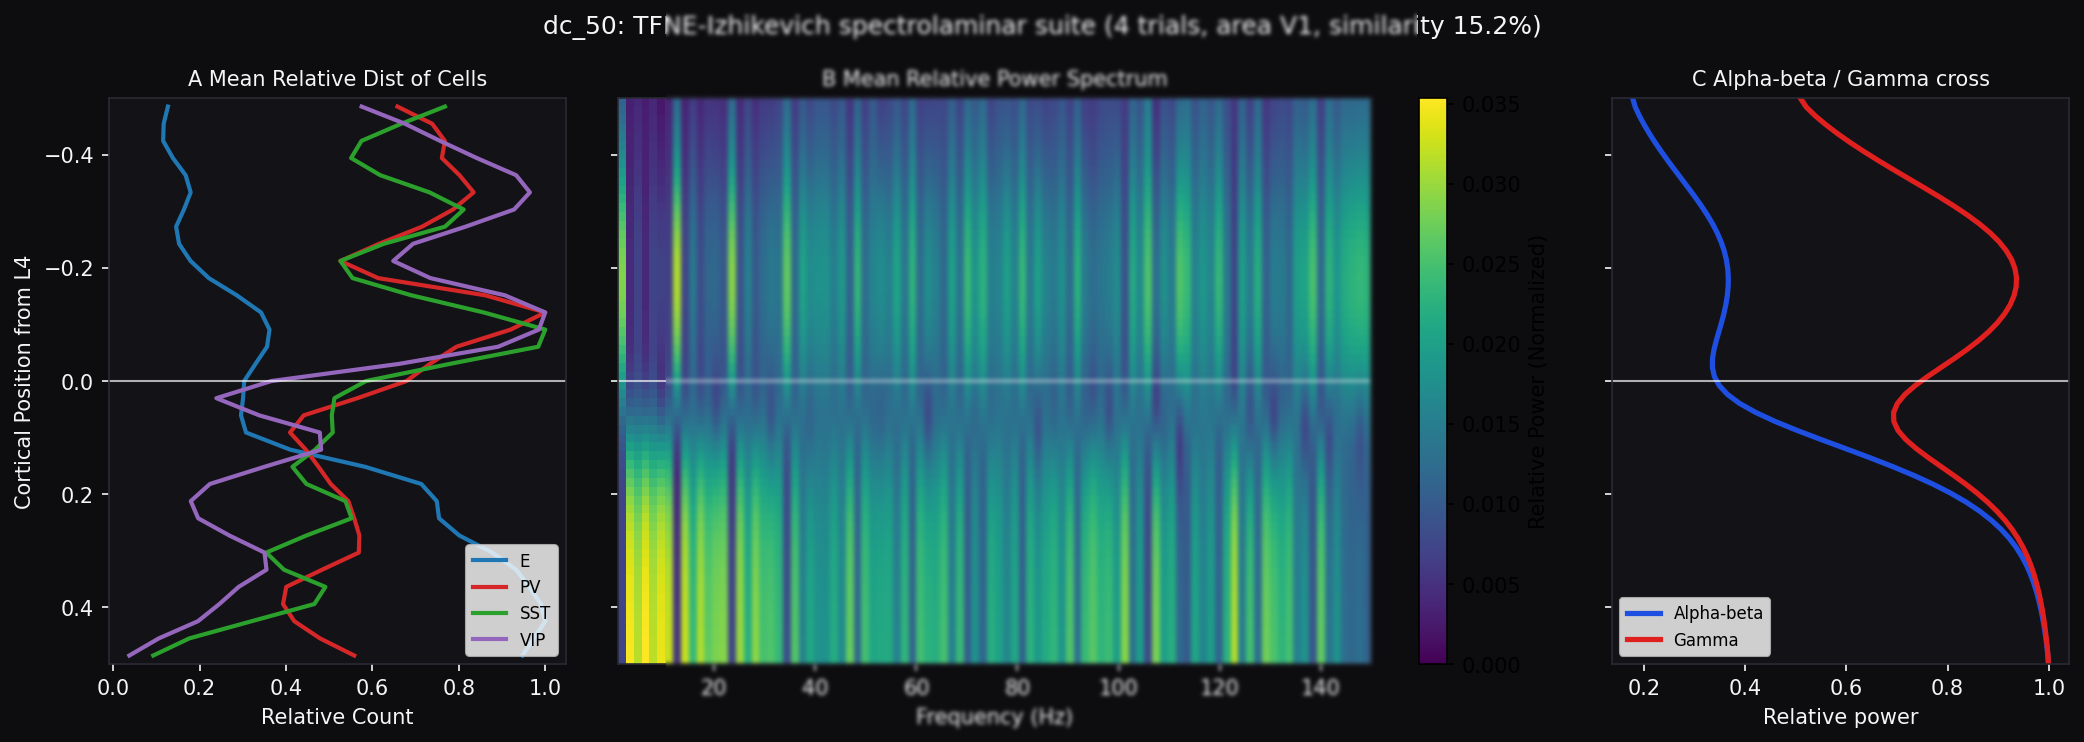
\includegraphics[width=0.75\textwidth]{spectrolaminar_suite_v2_dc50.png}
\caption{\small Spectrolaminar suite at $\mathrm{DC}_{\text{deep}}=50$ nA.
Mid-range drive; spectral structure stabilized by homeostatic plasticity.}
\end{figure}

\newpage
\subsubsection*{DC = 75 nA}
\begin{figure}[H]\centering
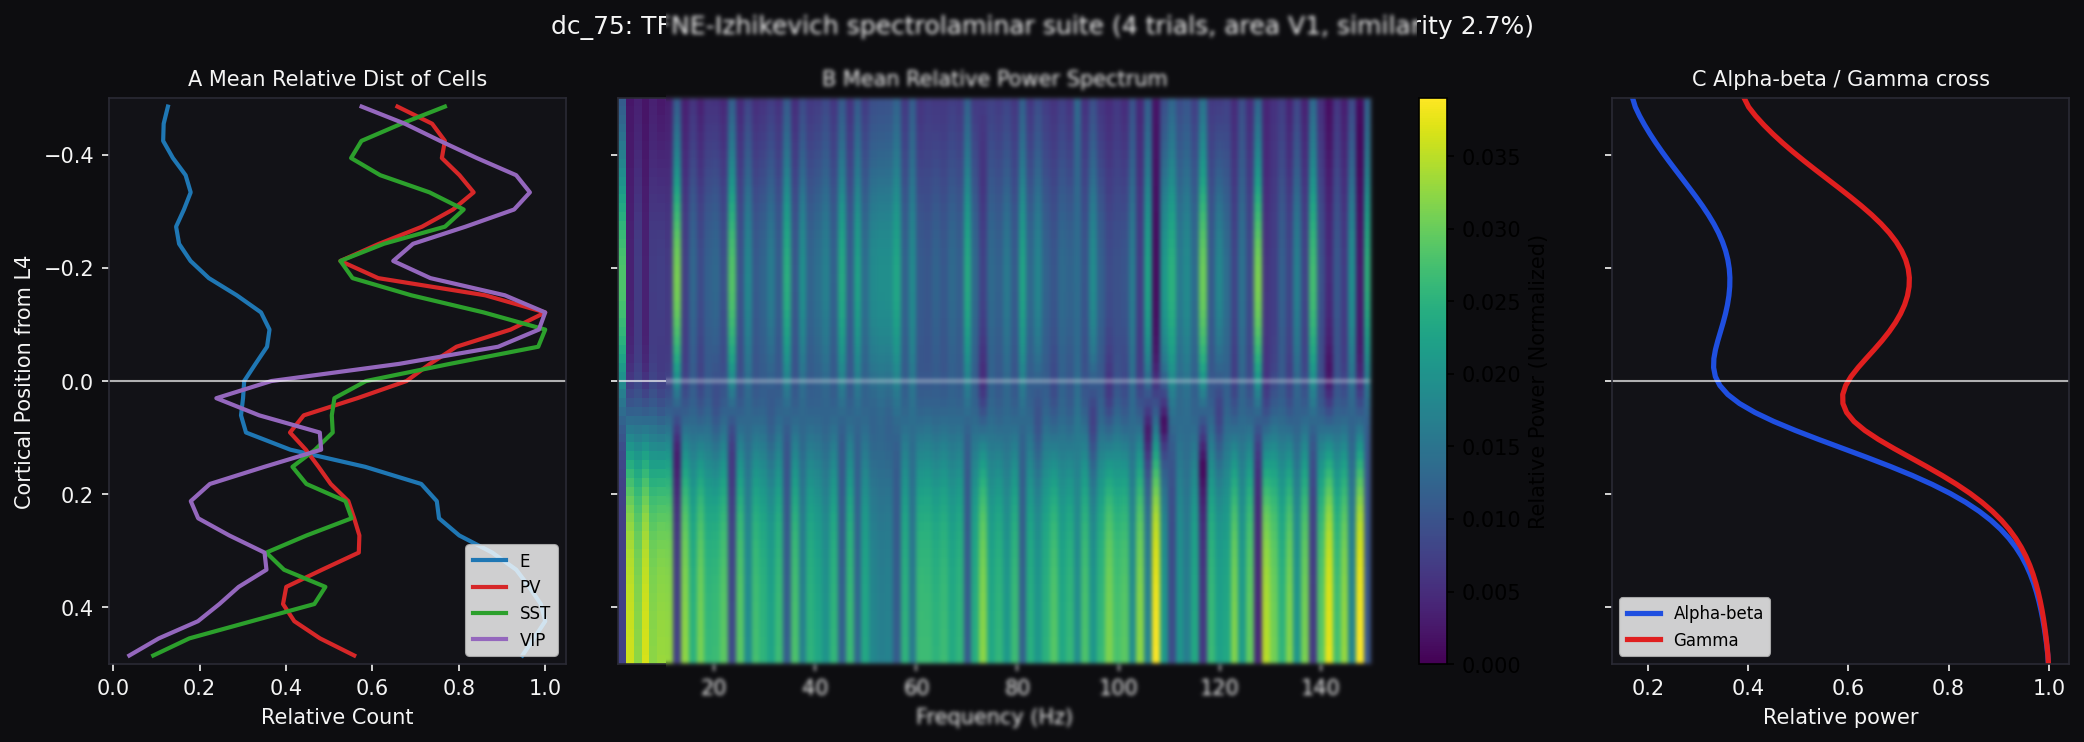
\includegraphics[width=0.75\textwidth]{spectrolaminar_suite_v2_dc75.png}
\caption{\small Spectrolaminar suite at $\mathrm{DC}_{\text{deep}}=75$ nA.
High drive; laminar organization persists despite strong E excitation.}
\end{figure}

\newpage
\subsubsection*{DC = 100 nA (maximum)}
\begin{figure}[H]\centering
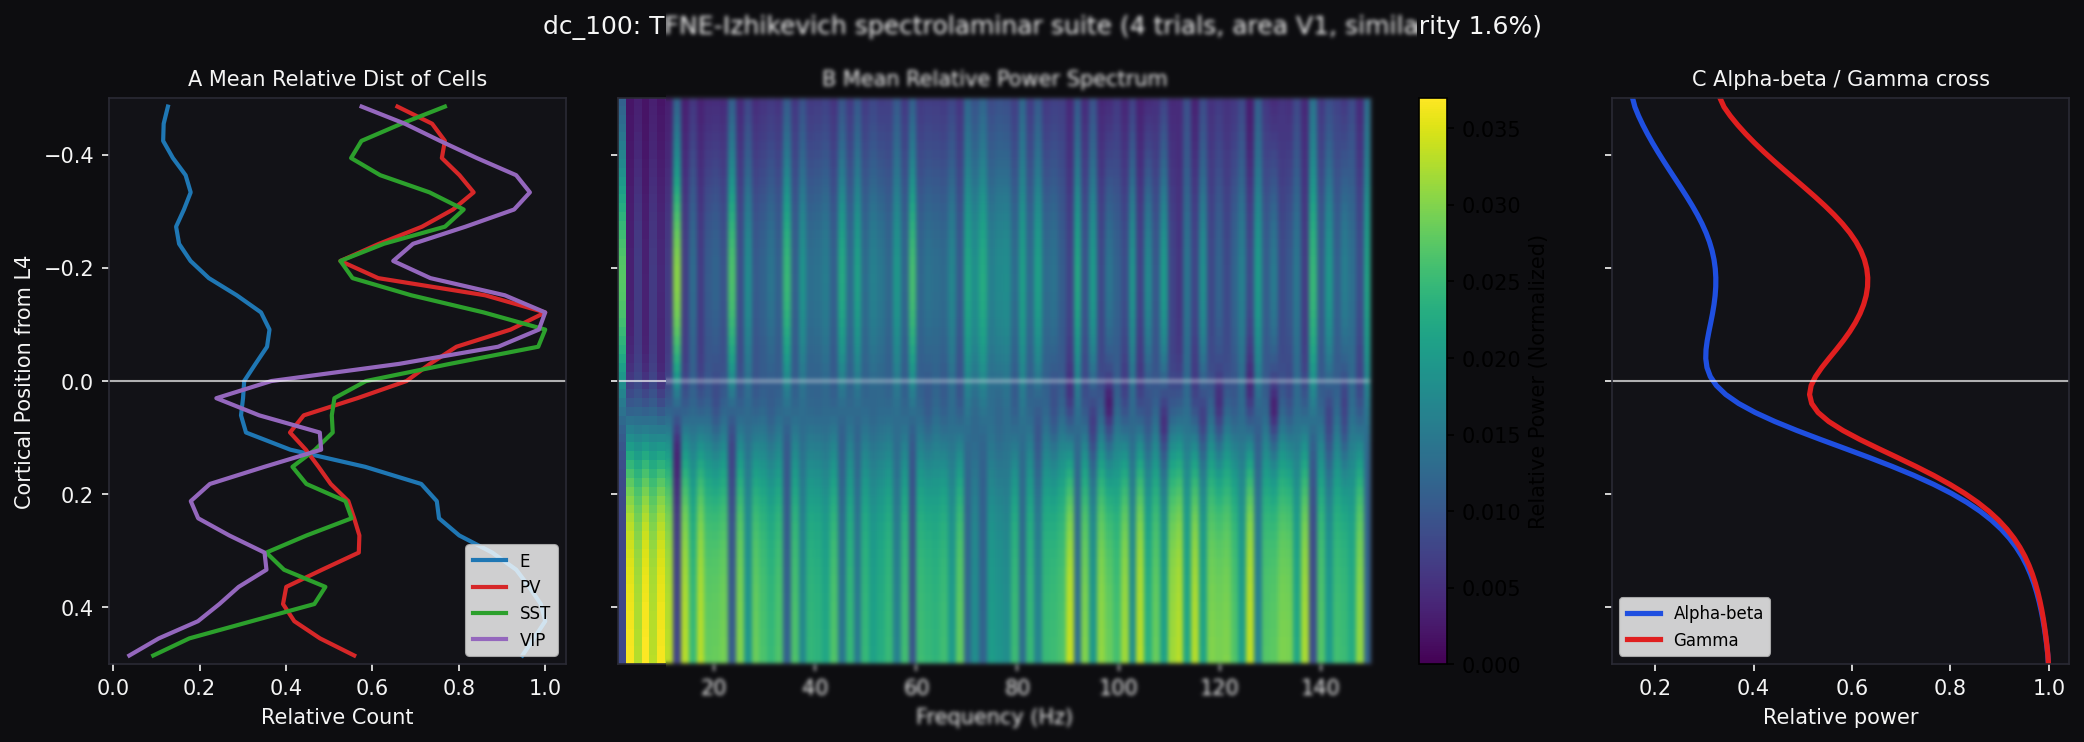
\includegraphics[width=0.75\textwidth]{spectrolaminar_suite_v2_dc100.png}
\caption{\small Spectrolaminar suite at maximum drive ($\mathrm{DC}_{\text{deep}}=100$ nA).
Despite strong deep drive, E/I homeostasis maintains balanced laminar profiles.}
\end{figure}

\section{EEG and MEG proxies}
\begin{figure}[H]\centering
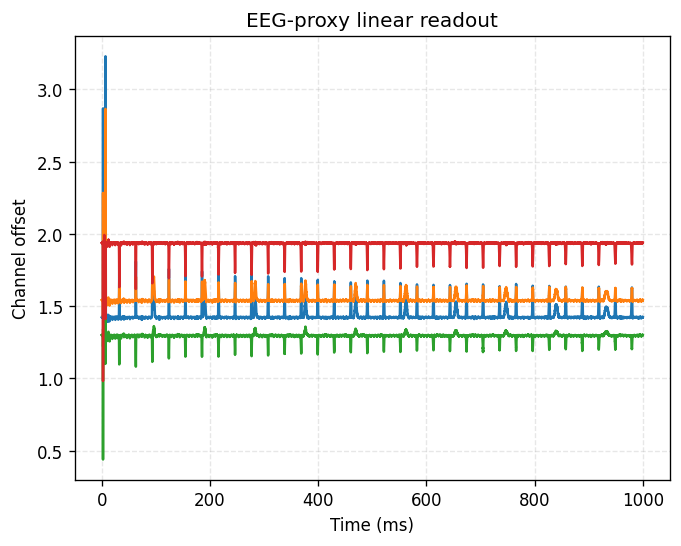
\includegraphics[width=0.48\textwidth]{05_eeg_proxy.png}\hfill
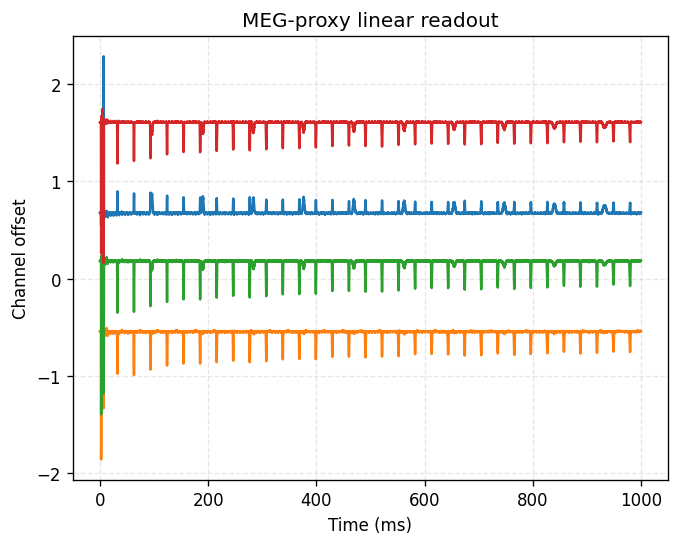
\includegraphics[width=0.48\textwidth]{06_meg_proxy.png}
\caption{Left: $\mathrm{eeg\_proxy}$ (linear leadfield projection to scalp electrodes).
Right: $\mathrm{meg\_proxy}$ (oriented-source magnetic projection). Both are proxy
readouts in relative units.}
\end{figure}

\section{Additional diagnostics}
\begin{figure}[H]\centering
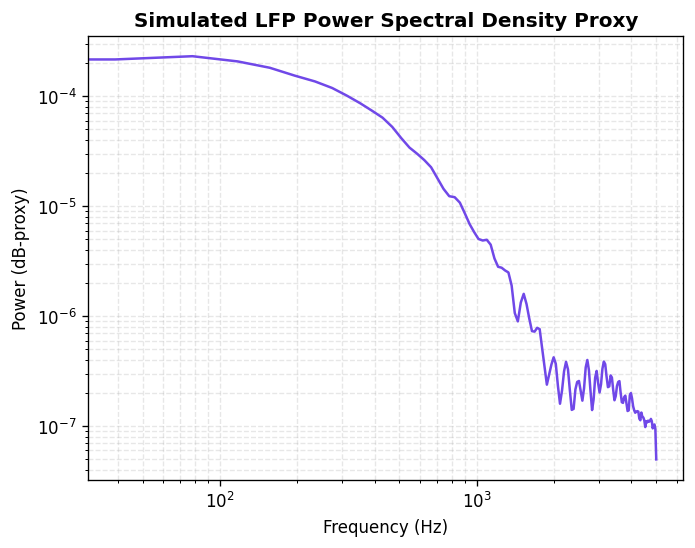
\includegraphics[width=0.6\textwidth]{11_psd.png}
\caption{Power spectral density proxy of the laminar field.}
\end{figure}

\section{Why the spectrolaminar suite is the preferred visualization}\label{sec:crossing}
The spectrolaminar suite normalizes each band across depth, exposing \emph{relative} laminar
organization that raw LFP amplitude---dominated by the densest/most-driven layers---obscures,
and it is robust to absolute-amplitude scaling (appropriate here, as all outputs are
uncalibrated proxies).

\textbf{Scope note on the laminar crossing.} The canonical spectrolaminar motif is
$\alpha/\beta$ power peaking in deep layers and $\gamma$ peaking superficially. In this
scaffold that crossing is \emph{readout- and scale-dependent}: it has been observed only via
an explicit $128$-contact \emph{normalized} projection at the full $N=10{,}000$ scale and does
not transfer to reduced surrogates. On the suite's default ($16$-contact) auto field used for
the figures above, the measured band fractions (Table~\ref{tab:metrics}) do \emph{not} reproduce
it---deep $\gamma$ fraction in fact rises with deep drive. We therefore report the monotonic
rate/power increase as the robust effect and treat the laminar crossing as an unvalidated,
scaffold-level observation, consistent with \texttt{claim\_level=computational\_scaffold}.

\section*{Scope statement}
All field outputs are computational proxies
(\texttt{claim\_level=computational\_scaffold}, \texttt{field\_solver\_status=linear\_solver},
\texttt{field\_claim\_level=proxy\_readout}, \texttt{physical\_amplitude\_calibrated=False}).
They are not physical EEG/MEG/LFP/CSD measurements and carry no calibrated amplitude.

\end{document}
